\documentclass[a5paper, 11pt]{extarticle}
\usepackage[utf8]{inputenc}
\usepackage[T1]{fontenc}
\usepackage{graphicx}
\usepackage{longtable}
\usepackage{tabularray}
\usepackage{wrapfig}
\usepackage{rotating}
\usepackage{float}
\usepackage[normalem]{ulem}
\usepackage{amsmath}
\usepackage{amssymb}
\usepackage{capt-of}
\usepackage{hyperref}
\usepackage{fontspec}
\usepackage[russian]{babel}
\usepackage{indentfirst}
\usepackage{MnSymbol}
\usepackage[
    left=10mm,
    right=10mm,
    top=15mm,
    bottom=15mm
]{geometry}
\usepackage{amsthm}
\usepackage{enumitem}
\usepackage{unicode-math}
\usepackage[math]{cellspace}
\usepackage{mathtools}

\setmainfont{PT Astra Serif}
\setmathfont{Latin Modern Math}
\setmathfont[range=\setminus]{Asana Math}
\setmathfont[range=\varnothing]{Asana Math}

\pagestyle{plain}

\theoremstyle{definition}
\newtheorem{theorem}{Теорема}[subsection]
\renewcommand{\thetheorem}{\arabic{theorem}}

\newtheorem*{theorem*}{Теорема}

\newtheorem{lemma}{Лемма}[subsection]
\renewcommand{\thelemma}{\arabic{lemma}}

\newtheorem{property}{Свойство}[subsection]
\renewcommand{\theproperty}{\arabic{property}}

\theoremstyle{definition}
\newtheorem{definition}{Определение}[subsection]
\renewcommand{\thedefinition}{\arabic{definition}}

\theoremstyle{definition}
\newtheorem*{definition*}{Определение}

\newtheorem{consequence}{Следствие}[subsection]
\makeatletter
\counterwithin{consequence}{property}
\counterwithin{consequence}{theorem}
\makeatother
\renewcommand{\theconsequence}{\arabic{consequence}}

\newtheorem*{consequence*}{Следствие}

\newtheorem{note}{Замечание}[subsection]
\makeatletter
\counterwithin{note}{property}
\counterwithin{note}{theorem}
\makeatother
\renewcommand{\thenote}{\arabic{note}}

\newtheorem*{note*}{Замечание}

\numberwithin{figure}{section}

\newcommand{\intersects}{\mathord{\bigcirc\kern-0.5em{\bigcirc}}}
\newcommand{\symdiff}{\medtriangleup}


\newcommand{\newpar}{$ $\par\nobreak\ignorespaces}
\renewenvironment{proof}{{\noindent\bfseries Доказательство.}}{\smallskip\newpar \hfill\textit{Что и требовалось доказать.}}
\usepackage[x11names]{xcolor}
\author{Daniil Shvalov}
\date{\today}
\title{}
\hypersetup{
    pdfauthor={Daniil Shvalov},
    pdftitle={},
    pdfkeywords={},
    pdfsubject={},
    pdflang={Russian}}


% Define math operators
\DeclareMathOperator{\rang}{rang}
\DeclareMathOperator{\Ima}{Im}
\DeclareMathOperator{\defect}{def}


% Draw line in matrix
\makeatletter
\renewcommand*\env@matrix[1][*\c@MaxMatrixCols c]{%
    \hskip -\arraycolsep
    \let\@ifnextchar\new@ifnextchar
    \array{#1}}
\makeatother

% Add new table align types
\newcommand{\PreserveBackslash}[1]{\let\temp=\\#1\let\\=\temp}
\newcolumntype{C}[1]{>{\PreserveBackslash\centering}p{#1}}

\setlist[itemize]{itemsep=0.5em,topsep=0em,parsep=0em}
\setlist[enumerate]{itemsep=0.5em,topsep=0em,parsep=0em}

\makeatletter
\def\thm@space@setup{\thm@preskip=1pt
    \thm@postskip=1pt}
\makeatother

\def\lets{%
    \mathord{\setbox0=\hbox{$\exists$}%
        \hbox{\kern 0.125\wd0%
            \vbox to \ht0{%
                \hrule width 0.75\wd0%
                \vfill%
                \hrule width 0.75\wd0}%
            \vrule height \ht0%
            \kern 0.125\wd0}%
    }%
}

\begin{document}

\hypersetup{linktoc = all, colorlinks = true, urlcolor = DodgerBlue4, citecolor = PaleGreen1, linkcolor = black}
\tableofcontents
\hypersetup{linktoc = all, colorlinks = true, urlcolor = DodgerBlue4, citecolor = PaleGreen1, linkcolor = blue}
\newpage

\section{Множества и отношения}

\subsection{Основные понятия}

\textbf{Множество} -- любая определенная совокупность объектов. Элементы множества различны и отличными друг от друга.

Под \textbf{множеством} понимают любой набор определенных и различимых между собой объектов, мыслимый как единое целое. Объекты, из которых составлено множество, называются его \textbf{элементами}.

Множества обычно обозначатся заглавными латинскими буквами: \(A, B, C, \ldots\). Элементы множества обозначаются строчными латинскими буквами: \(a, b, c, \ldots\).

Для обозначения того, что объект \(x\) является, либо не является элементом множества \(A\), используют символику:
\begin{itemize}
    \item \(x \in A\) -- объект \(x\) является элементом множества \(A\).
    \item \(x \notin A\) -- объект \(x\) не является элементом множества \(A\).
\end{itemize}

Множество, не содержащее ни одного элемента, называется \textbf{пустым} и обозначается символом \(\varnothing\).

Множество, из элементов которого составляют конкретное множество, называют \textbf{универсальным} и обозначают символом \(U\).

Множество \(U\) называется \textbf{универсальным} для данной задачи, если все рассматриваемые в этой задаче множества являются его подмножествами.

Множества можно изображать с помощью кругов, которые называются \textbf{кругами Эйлера} или \textbf{диаграммами Венна}. Универсальное множество принято обозначать прямоугольником.

Способы задания множества:
\begin{enumerate}
    \item перечислением всех элементов множества (в фигурных скобках через запятую):
          \[
              A = \{1, 2, 3, 4\};
          \]
    \item характеристическим предикатом, который описывает свойство всех элементов, входящих в множество. Характеристический предикат записывается после двоеточия или символа <<\(\mid\)>>:
          \[
              A = \{x: P(x)\}
              \quad
              \lor
              \quad
              A = \{x \mid P(x)\}
          \]
          где \(P(x)\) -- характеристический предикат.
\end{enumerate}

Обозначения числовых множеств:
\begin{itemize}
    \item \(\mathbb{N}\) -- множества натуральных чисел, \(\mathbb{N} = \{1, 2, 3, \ldots\}\);
    \item \(\mathbb{Z}\) -- множества целых чисел, \(\mathbb{Z} = \{\ldots, -2, -1, 0, 1, 2, \ldots\}\);
    \item \(\mathbb{Q}\) -- множество рациональных числе, \(\mathbb{Q} = \Big\{\dfrac{m}{n} (m \in \mathbb{Z}, n \in \mathbb{N})\Big\}\);
    \item \(\mathbb{R}\) -- множество действительных (вещественных) чисел;
    \item \(\mathbb{C}\) -- множество комплексных чисел.
\end{itemize}

\subsection{Сравнение множеств}

Множество \(A\) называется \textbf{подмножеством} множества \(B\) (множество \(A\) содержится в \(B\), множество \(B\) включает множество \(A\)), если каждый элемент множества \(A\) является элементом множества \(B\):
\[
    A \subseteq B
    \iff
    \forall x \in A \implies x \in B.
\]
\(B\) называется \textbf{надмножеством} множества \(A\).

Под определению пустое множество является подмножеством всех множеств:
\[
    \forall M \implies \varnothing \subseteq M.
\]
Универсальное множество содержит все множества:
\[
    \forall M \implies M \subseteq U.
\]

Два множества называют \textbf{равными}, если они являются подмножествами друг друга:
\[
    A = B
    \iff
    A \subseteq B \land B \subseteq A.
\]

Если \(A \subseteq B\) и \(A \neq B\), то множество \(A\) называется \textbf{собственным} подмножеством множества \(B\), а \(B\) -- \textbf{собственным} надмножеством \(A\).

Множества \(A\) и \(B\) \textbf{сравнимые}, если \(A \subseteq B \lor B \subseteq A\). Иначе множества называются \textbf{несравнимыми}.

\subsection{Свойства включения множеств}

\begin{property}
    \[
        \forall A \implies A \subseteq A.
    \]
\end{property}

\begin{property}
    \[
        \forall A, B : A \subseteq B \land B \subseteq A \implies A = B.
    \]
\end{property}

\begin{property}
    \[
        \forall A, B, C : A \subseteq B \land B \subseteq C \implies A \subseteq C.
    \]
\end{property}

\subsection{Мощность множества}

Говорят, что между множествами \(A\) и \(B\) установлено \textbf{взаимно-однозначное соответствие}, если каждому элементу множества \(A\) поставлен в соответствие один и только один элемент множества \(B\), и каждому элементу множества \(B\) поставлен в соответствие один и только один элемент множества \(A\):
\[
    A \sim B
    \iff
    \begin{dcases}
        \forall a \in A \mapsto !b \in B \\
        \forall b \in B \mapsto !a \in A
    \end{dcases}
\]

Два множества (конечных или бесконечных) имеют \textbf{одинаковую мощность}, если между этими множествами можно установить взаимно-однозначное соответствие. В этом случае говорят, что множества \(A\) и \(B\) \textbf{изоморфны}, имеют одинаковую \textbf{мощность}, или что они \textbf{равномощны}, и обозначают \(|A| = |B|\).

Множество \(A\) называется \textbf{конечным}, если у него нет равномощного собственного подмножества:
\[
    \forall B: B \subseteq A \land |B| = |A| \implies B = A.
\]
Для конечного множества используется запись \(|A| < \infty\).

Множество \textbf{бесконечно} тогда и только тогда, когда оно имеет одинаковую мощность с некоторым своим подмножеством, не совпадающим с самим этим множеством:
\[
    \exists B: B \subseteq A \land |B| = |A| \land B \neq A.
\]
То есть бесконечное множество равномощно некоторому своему собственному подмножеству. Для бесконечного множества используется запись \(|A| = \infty\).

Множество \(X\) называется \textbf{счетным}, если его мощность равна мощности множества натуральных чисел, т. е. \(|X| = |\mathbb{N}|\).

Говорят, что множество \(X\) -- множество \textbf{мощности континуума}, если его мощность равна мощности множества точек на отрезке \([0, 1]\).

\begin{theorem*}[Теорема Кантора о несчетности]
    Отрезок \([0, 1]\) несчетен, т. е.
    \[
        |[0, 1]| > |\mathbb{N}|.
    \]
\end{theorem*}

\subsection{Операции над множествами}

\textbf{Объединением} двух множеств называется множество, содержащее все элементы обоих множеств:
\[
    A \cup B = \{x \mid x \in A \lor x \in B\}.
\]

\begin{figure}[H]
    \centering
    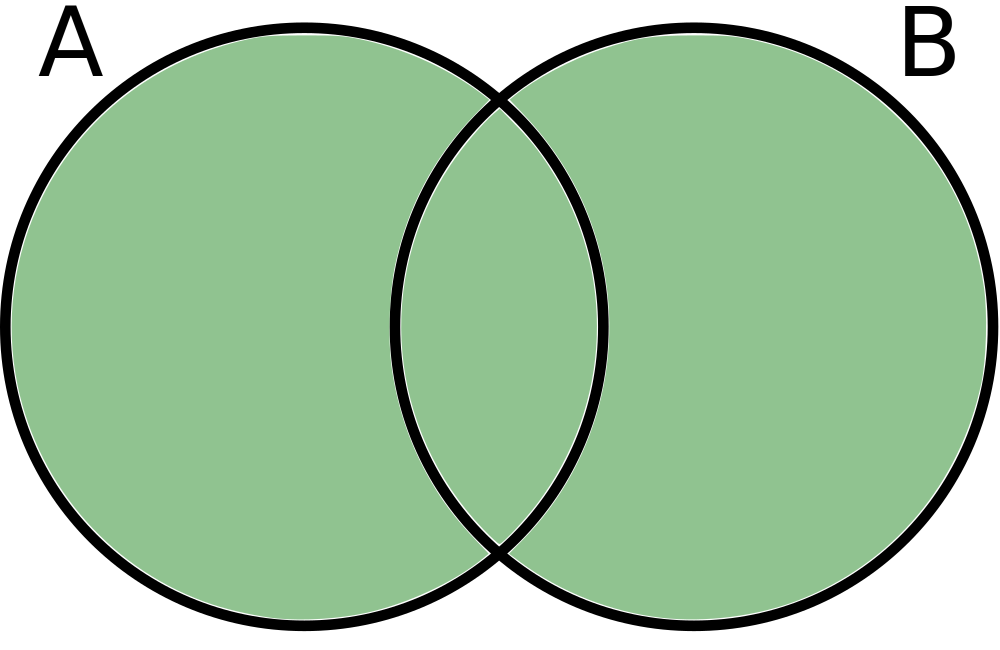
\includegraphics[width=0.5\textwidth]{images/set-combining.png}
    \caption{Объединение двух множеств}
\end{figure}

\textbf{Пересечением} двух множеств называется множество, состоящее из элементов, входящих в каждое из множеств \(A\) и \(B\):
\[
    A \cap B = \{x \mid x \in A \land x \in B\}.
\]

\begin{figure}[H]
    \centering
    
\includegraphics[width=0.5\textwidth]{images/set-intersection.png}
    \caption{Пересечение двух множеств}
\end{figure}

\textbf{Разностью} множеств \(A\) и \(B\) называется множество, состоящее из всех элементов множества \(A\), не содержащихся в множестве \(B\):
\[
    A \setminus B = \{x \mid x \in A \land x \notin B\}.
\]

\begin{figure}[H]
    \centering
    
\includegraphics[width=0.5\textwidth]{images/set-difference.png}
    \caption{Разность двух множеств}
\end{figure}

\textbf{Симметрической разностью} множеств \(A\) и \(B\) называется множество, состоящее из всех элементов множества \(A\), не содержащихся в множестве \(B\), и всех элементов множества \(B\), не содержащихся в множестве \(A\):
\[
    A \symdiff B = \{x \mid (x \in A \land x \notin B) \lor (x \notin A \land x \in B)\}.
\]

\begin{figure}[H]
    \centering
    
\includegraphics[width=0.5\textwidth]{images/set-sym-difference.png}
    \caption{Симметрическая разность двух множеств}
\end{figure}

\textbf{Дополнением} (дополнением до универсального множества \(U\)) множества \(A\) называется множество, состоящее из всех элементов универсального множества, не содержащихся в множестве \(A\):
\[
    \bar{A} = \{x \mid x \notin A\}.
\]

\begin{figure}[H]
    \centering
    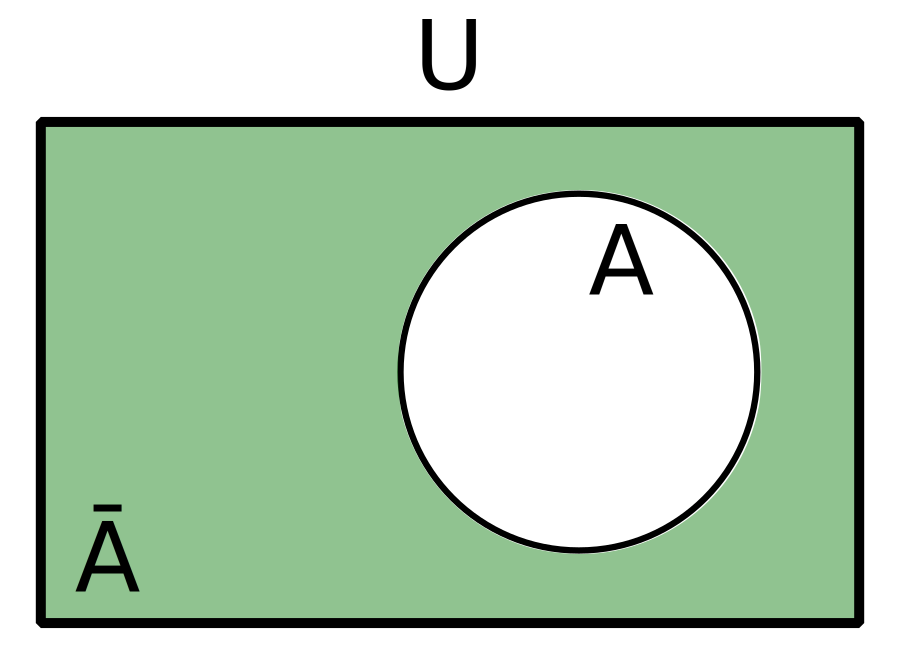
\includegraphics[width=0.55\textwidth]{images/set-complement.png}
    \caption{Дополнение множества}
\end{figure}

\subsection{Свойства операций над множествами}

\begin{property}[Идемпотентность]
    \[
        A \cup A = A;
        \qquad
        A \cap A = A.
    \]
\end{property}

\begin{property}[Коммутативность]
    \[
        A \cup B = B \cup A;
        \qquad
        A \cap B = B \cap A.
    \]
\end{property}

\begin{property}[Ассоциативность]
    \[
        A \cup (B \cup C) = (A \cup B) \cup C;
        \qquad
        A \cap (B \cap C) = (A \cap B) \cap C.
    \]
\end{property}

\begin{property}[Дистрибутивность]
    \[
        A \cup (B \cap C) = (A \cup B) \cap (A \cup C);
        \qquad
        A \cap (B \cup C) = (A \cap B) \cup (A \cap C).
    \]
\end{property}

\begin{property}[Поглощение]
    \[
        (A \cap B) \cup A = A;
        \qquad
        (A \cup B) \cap A = A.
    \]
\end{property}

\begin{property}[Свойства нуля]
    \[
        A \cup \varnothing = A;
        \qquad
        A \cap \varnothing = \varnothing.
    \]
\end{property}

\begin{property}[Свойства единицы]
    \[
        A \cup U = U;
        \qquad
        A \cap U = A.
    \]
\end{property}

\begin{property}[Инволютивность]
    \[
        \bar{\bar{A}} = A.
    \]
\end{property}

\begin{property}[Законы де Моргана]
    \[
        \overline{A \cap B} = \bar{A} \cup \bar{B};
        \qquad
        \overline{A \cup B} = \bar{A} \cap \bar{B}.
    \]
\end{property}

\begin{property}[Свойства дополнения]
    \[
        A \cup \bar{A} = U;
        \qquad
        A \cap \bar{A} = \emptyset.
    \]
\end{property}

\begin{property}[Свойство разности]
    \[
        A \setminus B = A \cap \bar{B}.
    \]
\end{property}

\begin{property}[Свойство симметрической разности]
    \[
        A \symdiff B = (A \setminus B) \cap (B \setminus A).
    \]
\end{property}

\subsection{Обобщенные тождества алгебры множеств}

\begin{property}[Обобщенная дистрибутивность]
    \[
        A \cap \bigcup_{i = 1}^n B_i = \bigcup_{i = 1}^n (A \cap B_i);
        \qquad
        A \cup \bigcap_{i = 1}^n B_i = \bigcap_{i = 1}^n (A \cup B_i).
    \]
\end{property}

\begin{property}[Обобщенный закон де Моргана]
    \[
        \overline{\bigcup_{i = 1}^n A_i} = \bigcap_{i = 1}^n \overline{A_i};
        \qquad
        \overline{\bigcap_{i = 1}^n A_i} = \bigcup_{i = 1}^n \overline{A_i}.
    \]
\end{property}

\subsection{Булеан}

Множество всех подмножеств \(A\) называется \textbf{булеаном} множества \(A\) и обозначается \(2^A\):
\[
    2^A = \{B \mid B \subseteq A\}.
\]

\begin{theorem*}
    Если множество \(A\) конечно, то \(|2^A| = 2^{|A|}\).
\end{theorem*}

\subsection{Методы доказательств теоретико-множественных тождеств}

\subsubsection{Метод двух включений}

Пусть левая часть теоретико-множественного тождества определяет множество \(X\), а правая часть -- множество \(Y\). Чтобы доказать равенство множеств \(X\) и \(Y\), достаточно доказать два включения \(X \subseteq Y\) и \(Y \subseteq X\), т. е. доказать, что
\[
    \forall x \in X \implies x \in Y
    \quad \land \quad
    \forall x \in Y \implies x \in X.
\]

Докажем этим методом тождество
\[
    A \symdiff B = (A \cup B) \setminus (A \cap B).
\]

Пусть \(x \in A \symdiff B\). Тогда, согласно определению симметрической разности
\begin{gather*}
    x \in (A \symdiff B) \implies
    x \in ((A \setminus B) \cup (B \setminus A)) \implies \\ \implies
    (x \in A \land x \notin B) \lor (x \in B \land x \notin A) \implies \\ \implies
    (x \in (A \cup B) \land x \notin (A \cap B)) \lor (x \in (A \cup B) \land x \notin (A \cap B)) \implies \\ \implies
    x \in (A \cup B) \land x \notin (A \cap B) \implies
    x \in ((A \cup B) \setminus (A \cap B)).
\end{gather*}

Таким образом доказано, что \(A \symdiff B \subseteq (A \cup B) \setminus (A \cap B)\). Докажем обратное включение \((A \cup B) \setminus (A \cap B) \subseteq A \symdiff B\):
\begin{gather*}
    x \in ((A \cup B) \setminus (A \cap B)) \implies
    x \in (A \cup B) \land x \notin (A \cap B) \implies \\ \implies
    (x \in A \land x \notin B) \lor (x \in B \land x \notin A) \implies \\ \implies
    x \in ((A \setminus B) \cup (B \setminus A)) \implies
    x \in (A \symdiff B).
\end{gather*}

Оба включения имеют место и тождество доказано.

\subsubsection{Метод эквивалентных преобразований}

Теоретико-множественные тождества можно доказывать, используя свойства операций над множествами. Для этого нужно преобразовать левую часть в правую, или правую -- в левую, или правую и левую часть в некоторое третье выражение.

Докажем этим методом тождество:
\[
    (A \cap B) \symdiff (A \cap C) = A \cap (B \symdiff C).
\]

Преобразуем левую часть к правой:
\begin{gather*}
    (A \cap B) \symdiff (A \cap C) = \\ =
    ((A \cap B) \cup (A \cap C)) \cap \overline{(A \cap B) \cap (A \cap C)} = \\ =
    (A \cap (B \cup C)) \cap (\overline{A \cap B} \cup \overline{A \cap C}) = \\ =
    (A \cap (B \cup C)) \cap (\bar{A} \cup \bar{B} \cup \bar{A} \cup \bar{C}) = \\ =
    (A \cap (B \cup C)) \cap (\bar{A} \cup \bar{B} \cup \bar{C}) = \\ =
    ((A \cap (B \cup C)) \cap \bar{A}) \cup ((A \cap (B \cup C)) \cap (\bar{B} \cup \bar{C})) = \\ =
    (B \cup C) \cap (A \cap (\bar{B} \cup \bar{C})) = \\ =
    (A \cap (B \cup C)) \cap (A \cap (\overline{B \cap C})) = \\ =
    A \cap ((B \cup C) \cap (\overline{B \cap C})) = \\ =
    A \cap (B \symdiff C).
\end{gather*}

\subsubsection{Метод характеристических функций}

Характеристическая функция \(\chi_A\) множества \(A\) для \(x \in U\) определяется следующим образом:
\[
    \begin{dcases}
        \chi_A(x) = 1, \quad x \in A \\
        \chi_A(x) = 0, \quad x \notin A
    \end{dcases}
\]
Для характеристической функции справедливы следующие тождества:
\begin{enumerate}
    \item \(\chi_A^2(x) = \chi_A(x)\);
    \item \(\chi_{A \cap B}(x) = \chi_A(x) \cdot \chi_B(x)\);
    \item \(\chi_{A \cup B}(x) = \chi_A(x) + \chi_B(x) - \chi_A(x) \cdot \chi_B(x)\);
    \item \(\chi_{\bar{A}} = 1 - \chi_A(x)\);
    \item \(\chi_{A \setminus B}(x) = \chi_A(x) - \chi_A(x) \cdot \chi_B(x)\);
    \item \(\chi_{A \symdiff B} = \chi_A(x) + \chi_B(x) - 2 \cdot \chi_A(x) \cdot \chi_B(x)\).
\end{enumerate}

Докажем этим методом тождество
\[
    (A \symdiff B) \cap C = (A \cap C) \symdiff (B \cap C).
\]

С одной стороны,
\begin{gather*}
    \chi_{(A \symdiff B) \cap C}(x) =
    \chi_{(A \symdiff B)}(x) \chi_C(x) = \\ =
    \big(\chi_A(x) + \chi_B(x) - 2 \chi_A(x) \chi_B(x)\big) \chi_C(x) = \\ =
    \chi_A(x) \chi_C(x) + \chi_B(x) \chi_C(x) - 2 \chi_A(x) \chi_B(x) \chi_C(x).
\end{gather*}

С другой стороны,
\begin{gather*}
    \chi_{(A \cap C) \symdiff (B \cap C)}(x) =
    \chi_{(A \cap C)}(x) + \chi_{(B \cap C)}(x) - 2 \chi_{(A \cap C)}(x) \chi_{(B \cap C)}(x) = \\ =
    \chi_A(x) \chi_C(x) + \chi_B(x) \chi_C(x) - 2 \chi_A(x) \chi_C(x) \chi_B(x) \chi_C(x) = \\ =
    \chi_A(x) \chi_C(x) + \chi_B(x) \chi_C(x) - 2 \chi_A(x) \chi_B(x) \chi_C(x).
\end{gather*}

Так как \(\chi_{(A \symdiff B) \cap C}(x) = \chi_{(A \cap C) \symdiff (B \cap C)}(x)\), тождество доказано.

\subsection{Упорядоченные пары и наборы}

\((a, b)\) -- упорядоченная пара объектов \(a\) и \(b\).

Равенство упорядоченных пар определяется следующим образом:
\[
    (a, b) = (c, d) \iff a = c \land b = d.
\]

Вообще говоря, \((a, b) \neq (b, a)\).

\((a_1, a_2, \ldots, a_n)\) -- упорядоченный набор из \(n\) элементов (\(n\)-ка, кортеж или (конечная) последовательность).

\(|(a_1, a_2, \ldots, a_n)|\) -- длина набора, т. е. количество элементов в наборе.

\begin{theorem*}
    Два набора одной длины равны, если равны их соответствующие элементы
    \[
        \forall n (a_1, \ldots, a_n) = (b_1, \ldots, b_n) \iff a_1 = b_1 \land \ldots \land a_n = b_n.
    \]
\end{theorem*}

\subsection{Прямое произведение множеств}

Прямым (декартовым) произведением двух множества \(A\) и \(B\) называется множество всех упорядоченных пар, в которых первый элемент принадлежит \(A\), а второй принадлежит \(B\):
\[
    A \times B = \{(a, b) \mid a \in A \land b \in B\}.
\]
\[
    A \times B \neq B \times A.
\]

\begin{theorem*}
    Для конечных множества \(A\) и \(B\)
    \[
        |A \times B| = |A| \cdot |B|.
    \]
\end{theorem*}

Понятие прямого произведения допускает обобщение. Прямое произведение множеств \(A_1, \ldots, A_n\) -- это множество наборов (кортежей):
\[
    A_1 \times \ldots \times A_n
    =
    \{(a_1, \ldots, a_n) \mid a_1 \in A_1 \land \ldots \land a_n \in A_n\}.
\]
Множества \(A_i\) необязательно различны.

Степенью множества \(A\) называется его \(n\)-кратное произведение самого на себя:
\[
    A^n = \underbrace{A \times \ldots \times A}_{n-\text{раз}};
    \qquad
    |A^n| = |A|^n.
\]

\subsection{Бинарные отношения}

Бинарным отношением между множествами \(A\) и \(B\) называется такая тройка \(\langle A, B, R \rangle\), где \(R\) -- подмножество прямого произведения \(A\) и \(B\):
\[
    R \subset A \times B,
\]
Эти множества именуют следующим образом:
\begin{itemize}
    \item \(R\) -- график отношения;
    \item \(A\) -- область отправления;
    \item \(B\) -- область прибытия.
\end{itemize}

Область определения отношения:
\[
    \text{Dom} R = \{a \in A \mid \exists b \in B : ((a, b) \in R)\}.
\]

Область значений:
\[
    \text{Im} R = \{b \in B \mid \exists a \in A : ((a, b) \in R)\}.
\]

Если \(A = B\) (т. е. \(R \subset A^2\)), то говорят, что \(R\) есть отношение на множестве \(A\).

Для бинарных отношений обычно используется \textbf{инфиксная} форма записи:
\[
    aRb \iff (a, b) \in R \subset A \times B.
\]

Инфиксная форма позволяет более кратко записывать некоторые формы утверждений относительно отношений:
\[
    aRbRc \iff (a, b) \in R \land (b, c) \in R
\]

Обратное отношение:
\[
    R^{-1} = \{(b, a) \mid (a, b) \in R\} \subset B \times A.
\]

Дополнение отношения:
\[
    \bar{R} = \{(a, b) \mid (a, b) \notin R\} \subset A \times B.
\]

Тождественное отношение:
\[
    I = \{(a, a) \mid a \in A\} \subset A^2.
\]

Универсальное отношение:
\[
    U = \{(a, b) \mid A \in A \land b \in B\} = A \times B.
\]

\subsection{Многоместные отношения}

\(n\)-местное (\(n\)-арное) отношение \(R\) -- это подмножество прямого произведения \(n\) множеств, т. е. множество упорядоченных наборов (кортежей):
\[
    R \subset A_1 \times \ldots \times A_n
    \iff
    \{(a_1, \ldots, a_n) \mid a_1 \in A_1 \land \ldots \land a_n \in A_n\},
\]
где \(n\) -- вместимость (длина кортежей отношения).

\subsection{Композиция отношений}

Пусть \(R_1 \subset A \times B\) -- отношение между множествами \(A\) и \(B\), а \(R_2 \subset B \times C\) -- отношение между множествами \(B\) и \(C\). \textbf{Композицией} двух отношений \(R_1\) и \(R_2\) называется отношение \(R \subset A \times C\) между множествами \(A\) и \(C\), определяется следующим образом:
\[
    R = R_1 \circ R_2 =
    \{(a, c) \mid a \in A \land c \in C \land \exists b \in B : (a R_1 b \land b R_2 c)\}.
\]

Композиция отношений ассоциативна, т. е.
\begin{gather*}
    \forall R_1 \subset A \times B, R_2 \subset B \times C, R_3 \subset C \times D
    \implies \\ \implies
    (R_1 \circ R_2) \circ R_3 = R_1 \circ (R_2 \circ R_3).
\end{gather*}

Композиция отношений на множестве \(A\) является отношением на множестве \(A\).

Степенью отношения \(R\) на множестве \(A\) называется его \(n\)-кратная композиция с самим собой:
\[
    R^n = \underbrace{R \circ \ldots \circ R}_{n-\text{раз}}.
\]


\subsection{Способы задания бинарных отношений}

\subsubsection{Матричный способ}

Отношение \(R \subset A \times B\) задается с помощью прямоугольной таблицы (матрицей), состоящей из нулей и единиц, в которой строки -- первые координаты, а столбцы -- вторые, причем на пересечении \(i\)-ой строки и \(j\)-го столбца будет стоять \(1\), если имеется отношение \(a_i R b_j\), и \(0\) в противном случае.

Рассмотрим пример. Пусть
\[
    A = \{1, 2, 3\},
    \quad
    B = \{2, 3, 4, 5, 6\}.
\]

Отношение
\[
    R = \{(1, 2), (1, 4), (2, 3), (3, 4), (3, 6)\}.
\]

Отношение можно записать в виде матрицы:
\[
    [R] =
    \begin{pmatrix}
        1 & 0 & 1 & 0 & 0 \\
        0 & 1 & 0 & 0 & 0 \\
        0 & 1 & 0 & 0 & 1
    \end{pmatrix}
\]

Матрица \textbf{универсального} (полного) отношения -- это квадратная матрица, состоящая только из единиц.

Матрица \textbf{тождественного} (диагонального) отношения -- это квадратная матрица, элементами главной диагонали которой являются единицы, а остальные элементы равны нулю.

Матрица \textbf{пустого} отношения -- это квадратная матрица, состоящая только из нулей.

Матрица \textbf{обратного} отношения \(R^{-1}\) для отношения \(R\) -- это транспортированная матрица отношения \(R\).

\subsubsection{С помощью ориентированного графа}

Элементы множеств \(A\) и \(B\) изображаются в виде точек на плоскости (вершины двудольного графа), а упорядоченные пары --  линией со стрелкой (дуги ориентированного графа), которая направленна от \(a\) к \(b\), если \(aRb\).

Рассмотрим пример. Пусть
\[
    A = \{1, 2, 3\},
    \quad
    B = \{2, 3, 4, 5, 6\}.
\]

Отношение
\[
    R = \{(1, 2), (1, 4), (2, 3), (3, 3), (3, 6)\}.
\]
\begin{figure}[H]
    \centering
    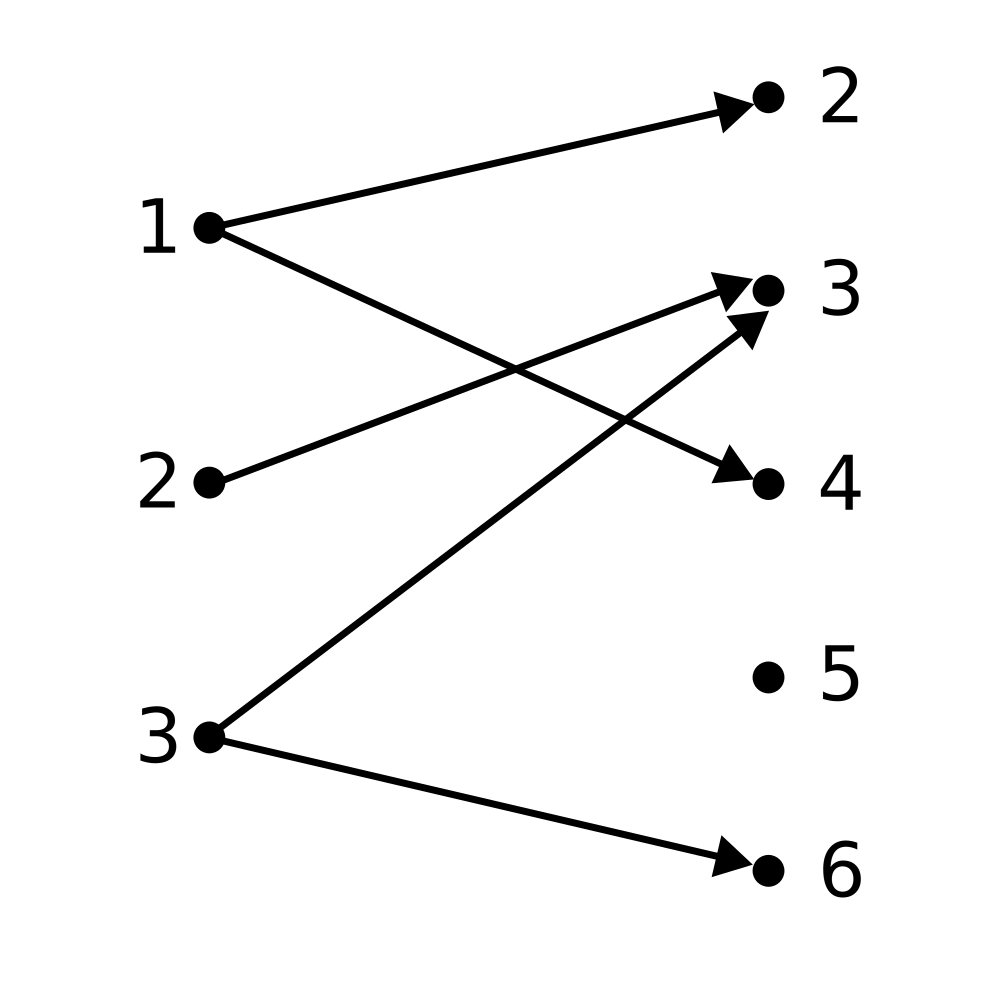
\includegraphics[width=0.5\textwidth]{images/relation-graph.png}
    \caption{Отношение в виде ориентированного графа}
\end{figure}

\subsection{Способы задания композиции отношений}

\subsubsection{Матричный способ}

Матрица композиции отношений \(R \circ S\) получается как произведение матриц отношений \(R\) и \(S\) с дальнейшей заменой отличных от нуля элементов единицами.

Пусть
\begin{gather*}
    R = \{(1, 2), (2, 1), (2, 2), (3, 3), (3, 4)\},
    \\
    S = \{(1, 1), (1, 2), (2, 3), (2, 5), (3, 2), (3, 4), (4, 2), (4, 3)\}.
\end{gather*}

Тогда композиция равна
\begin{gather*}
    [R \circ S] =
    \begin{pmatrix}
        0 & 1 & 0 & 0 \\
        1 & 1 & 0 & 0 \\
        0 & 0 & 1 & 1
    \end{pmatrix}
    \times
    \begin{pmatrix}
        1 & 1 & 0 & 0 & 0 \\
        0 & 0 & 1 & 0 & 1 \\
        0 & 1 & 0 & 1 & 0 \\
        0 & 1 & 1 & 0 & 0
    \end{pmatrix}
    = \\ =
    \begin{pmatrix}
        0 & 0 & 1 & 0 & 1 \\
        1 & 1 & 1 & 0 & 1 \\
        0 & 2 & 1 & 1 & 0
    \end{pmatrix}
    =
    \begin{pmatrix}
        0 & 0 & 1 & 0 & 1 \\
        1 & 1 & 1 & 0 & 1 \\
        0 & 1 & 1 & 1 & 0
    \end{pmatrix}
\end{gather*}

\[
    R \circ S = \{(1, 3), (1, 5), (2, 1), (2, 2), (2, 3), (2, 5), (3, 2), (3, 3), (3, 4)\}.
\]

\subsubsection{С помощью ориентированных графов}

Пусть \(R \subset A \times B\) и \(S \subset B \times C\). Чтобы получить граф \(T = R \circ S\), надо к графу отношения \(R\) добавить граф отношения \(S\). Граф композиции отношений получим, если исключим вершины которые являются элементами множества \(B\).

Рассмотрим пример. Пусть
\begin{gather*}
    R = \{(1, 2), (2, 1), (2, 2), (3, 3), (3, 4)\}, \\
    S = \{(1, 1), (1, 2), (2, 3), (2, 5), (3, 2), (3, 4), (4, 2), (4, 3)\}.
\end{gather*}

\begin{figure}[H]
    \centering
    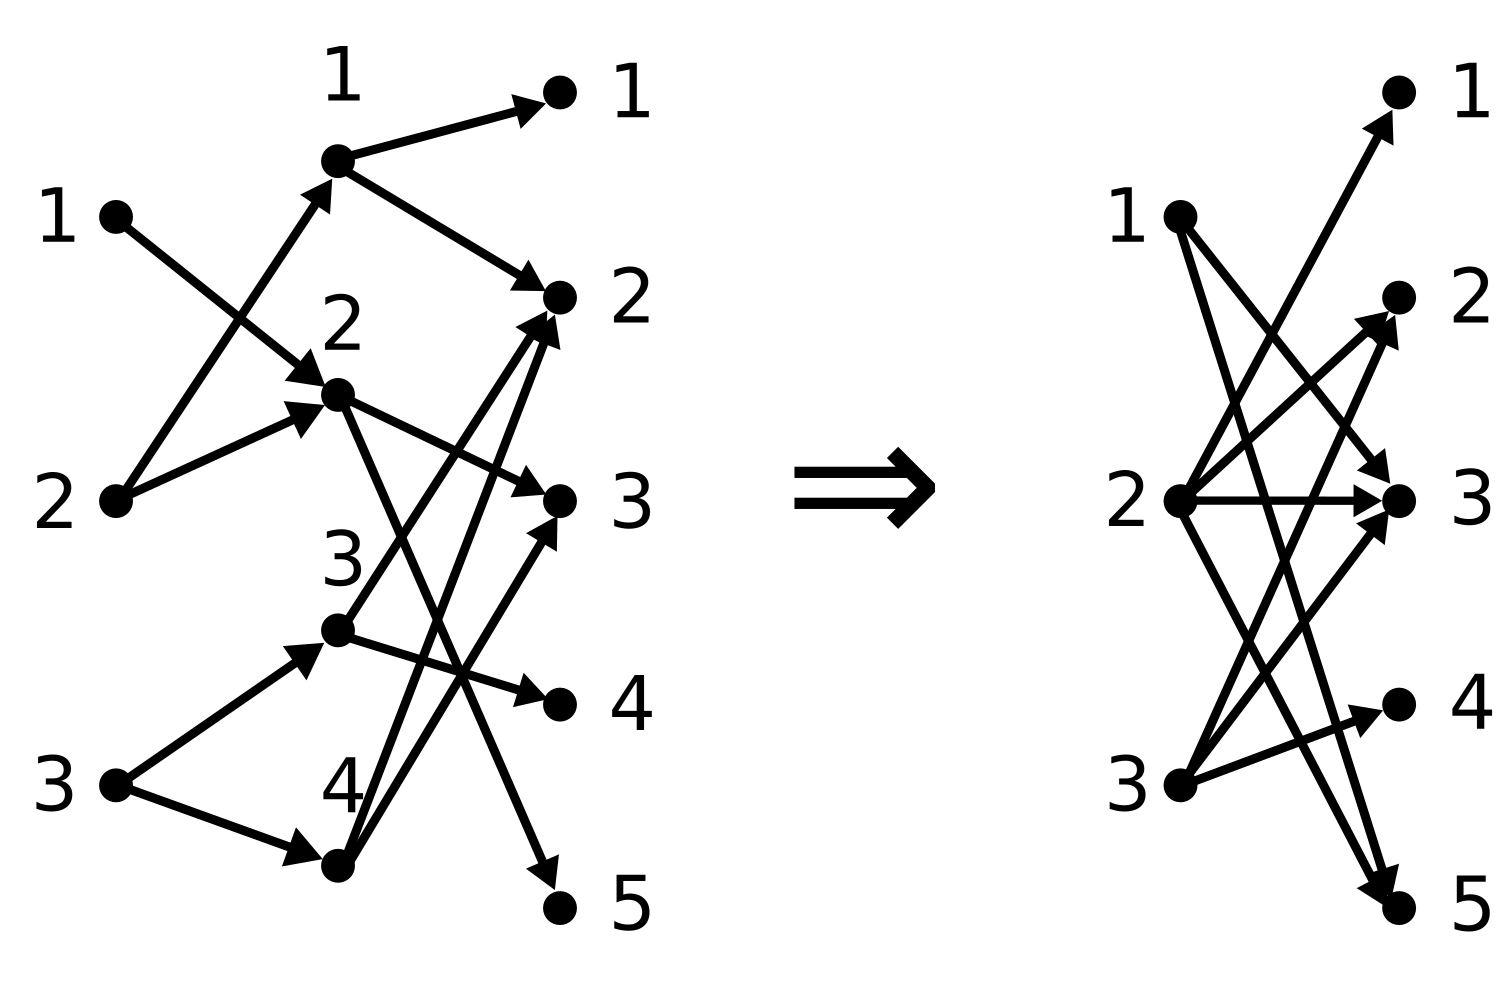
\includegraphics[width=0.8\textwidth]{images/composition-graph.png}
    \caption{Композиция в виде ориентированного графа}
\end{figure}

\subsection{Свойства бинарных отношений}

Бинарное отношение \(R\) на множестве \(A\) называется
\begin{itemize}
    \item \textbf{рефлексивным}, если
          \[
              \forall x \in A : (x, x) \in R;
          \]
    \item \textbf{антирефлексивным}, если
          \[
              \forall x \in A : (x, x) \notin R;
          \]
    \item \textbf{симметричным}, если
          \[
              \forall x, y \in A : (x, y) \in R \implies (y, x) \in R ;
          \]
    \item \textbf{антисимметричным}, если
          \[
              \forall x, y \in A : (x, y) \in R \land (y, x) \in R \implies x = y;
          \]
    \item \textbf{транзитивным}, если
          \[
              \forall x, y, z \in A : (x, y) \in R \land (y, z) \in R \implies (x, z) \in R;
          \]
    \item \textbf{линейным} (полным), если
          \[
              \forall x, y \in A : x = y \lor (x, y) \in R \lor (y, x) \in R.
          \]
\end{itemize}

\begin{theorem*}
    Пусть \(R \subset A \times A\) -- отношение на \(A\). Тогда
    \begin{itemize}
        \item \(R \text{ рефлексивно } \iff I \subset R\);
        \item \(R \text{ антирефлексивно } \iff R \cap I = \varnothing\);
        \item \(R \text{ симметрично } \iff R = R^{-1}\);
        \item \(R \text{ антисимметрично } \iff R \cap R^{-1} = I\);
        \item \(R \text{ транзитивно } \iff R \circ R \subset R\);
        \item \(R \text{ линейно } \iff R \cup I \cup R^{-1} = U\).
    \end{itemize}
\end{theorem*}

\subsection{Ядро отношения}

Если \(R \subset A \times B\) -- отношение между множествами \(A\) и \(B\), то композиция \(R \circ R^{-1}\) называется \textbf{ядром} отношения \(R\) и обозначается \(\text{ker} R\):
\[
    \text{ker} R = R \circ R^{-1}.
\]

Ядро отношения \(R\) между \(A\) и \(B\) является отношением на \(A\):
\[
    R \subset A \times B \implies \text{ker} R \subset A^2.
\]

\begin{theorem*}
    Ядро любого отношения рефлексивно и симметрично на области определения.
\end{theorem*}

\subsection{Замыкание отношений}

Пусть \(R\) и \(R^\times\) -- отношения на множестве \(M\). Отношение \(R^\times\) называется замыканием \(R\) относительно свойства \(C\), если
\begin{enumerate}
    \item \(R^\times\) обладает свойством \(C\): \(C(R^\times)\);
    \item \(R^\times\) является надмножеством \(R\): \(R \subset R^\times\);
    \item \(R^\times\) является наименьшим таким объектом:
          \[
              C(R^{\times \times}) \land R \subset R^\times \implies R^\times \subset R^{\times \times}.
          \]
\end{enumerate}

\begin{theorem*}
    Пусть \(R\) -- отношение на множестве \(M\). Тогда
    \begin{itemize}
        \item \(R \cup I\) есть рефлексивное замыкание \(R\);
        \item \(R \cup R^{-1}\) есть симметричное замыкание \(R\);
        \item если \(M\) -- конечное множество, содержащее \(n\) элементов, то отношение
              \[
                  R \cup R^2 \cup R^3 \cup \ldots \cup R^n
              \]
              есть транзитивное замыкание \(R\).
    \end{itemize}
\end{theorem*}

\subsection{Функциональные отношения}

Пусть \(f\) -- отношение между \(A\) и \(B\) такое, что
\[
    \forall a : (a, b) \in f \land (a, c) \in f \implies b = c.
\]

Такое свойство отношение называется \textbf{однозначностью} или \textbf{функциональным}, а само отношение называется \textbf{функцией} из \(A\) в \(B\).
\[
    f: A \to B \quad \text{или} \quad A \stackrel{f}{\to} B.
\]

\[
    b = f(a) \iff (a, b) \in f.
\]

\subsection{Тотальные и частичные функции}

\[
    \text{Dom} f \subset A;
    \qquad
    \text{Im} f \subset B
\]

Если \(\text{Dom} f = A\), то функция называется \textbf{тотальной}, а если \(\text{Dom} f \neq A\), то \textbf{частичной}.

\subsection{Инъекция, сюрьекция и биекция}

Пусть \(f: A \to B\), тогда функция \(f\) называется
\begin{itemize}
    \item \textbf{инъективной} (или инъекцией), если
          \[
              b = f(a_1) \land b = f(a_2) \implies a_1 = a_2;
          \]
    \item \textbf{сюрьективной} (или сюрьекция), если
          \[
              \forall b \in B \; \exists a \in A : b = f(a);
          \]
    \item \textbf{биективной} (или биекцией), если она инъективная или сюрьективная.
\end{itemize}

\subsection{Отношения эквивалентности}

Отношение называется отношением \textbf{эквивалентности} (эквивалентностью), если оно рефлексивно, симметрично и транзитивно. Эквивалентности обозначают символами \(E\), \(\sim\) (тильда) и \(=\):
\[
    xEy,
    \quad
    x \sim y,
    \quad
    x = y.
\]

Рассмотрим пример. Отношение равенства \(x = y\) является эквивалентностью на любом множестве \(A\), так как оно
\begin{itemize}
    \item рефлексивно (\(x = x\));
    \item симметрично (\(x = y \implies y = x\));
    \item транзитивно (\(x = y, y = z \implies x = z\)).
\end{itemize}

\subsection{Классы эквивалентности}

Пусть \(E\) -- отношение эквивалентности на множестве \(A\). \textbf{Классом эквивалентности} элемента \(x \in A\) называется подмножество элементов множества \(A\), эквивалентных \(x\):
\begin{gather*}
    E(x) = \{y \in A \mid xEy\}
    \\ \text{или} \\
    [x]_E = \{y \in A \mid y \equiv x\}.
\end{gather*}

\subsection{Фактормножества}

Если \(E\) -- отношение эквивалентности на множестве \(A\), то множество классов эквивалентности называется \textbf{фактормножеством} множества \(A\) относительно эквивалентности \(E\) и обозначается \(A \slash E\):
\[
    A \slash E = \{E(x) \mid x \in A\}
    \quad
    \text{или}
    \quad
    A \slash E = \{[x]_E\}_{x \in A}.
\]

\subsection{Отношения порядка}

Антисимметричное транзитивное отношение называется \textbf{отношением порядка}. Отношение порядка в общем случае обозначается символом \(\prec\). Отношение порядка может обладать также дополнительными свойствами, которые сведены в следующую таблицу:

\begin{center}
    \renewcommand*{\arraystretch}{1.5}
    \begin{longtable}{|C{0.45\textwidth}|C{0.45\textwidth}|}
        \hline
        Дополнительное свойство, которым обладает отношением порядка & Название отношения порядка, обладающего дополнительным свойством \\
        \hline
        рефлексивность                                               & отношение нестрогого порядка \(\leq\)                            \\
        \hline
        антирефлексивность                                           & отношение строгого порядка \(<\)                                 \\
        \hline
        линейность                                                   & отношение линейного порядка                                      \\
        \hline
        не обладает свойством линейности                             & отношение частичного порядка                                     \\
        \hline
    \end{longtable}
\end{center}

Множества, на котором задано отношение частичного порядка, называется \textbf{частично упорядоченным}.

Множество, на котором задано отношение линейного порядка, называется \textbf{линейно упорядоченным}.

\end{document}
